% Options for packages loaded elsewhere
\PassOptionsToPackage{unicode}{hyperref}
\PassOptionsToPackage{hyphens}{url}
\PassOptionsToPackage{dvipsnames,svgnames,x11names}{xcolor}
%
\documentclass[
  letterpaper,
  DIV=11,
  numbers=noendperiod]{scrreprt}

\usepackage{amsmath,amssymb}
\usepackage{lmodern}
\usepackage{iftex}
\ifPDFTeX
  \usepackage[T1]{fontenc}
  \usepackage[utf8]{inputenc}
  \usepackage{textcomp} % provide euro and other symbols
\else % if luatex or xetex
  \usepackage{unicode-math}
  \defaultfontfeatures{Scale=MatchLowercase}
  \defaultfontfeatures[\rmfamily]{Ligatures=TeX,Scale=1}
\fi
% Use upquote if available, for straight quotes in verbatim environments
\IfFileExists{upquote.sty}{\usepackage{upquote}}{}
\IfFileExists{microtype.sty}{% use microtype if available
  \usepackage[]{microtype}
  \UseMicrotypeSet[protrusion]{basicmath} % disable protrusion for tt fonts
}{}
\makeatletter
\@ifundefined{KOMAClassName}{% if non-KOMA class
  \IfFileExists{parskip.sty}{%
    \usepackage{parskip}
  }{% else
    \setlength{\parindent}{0pt}
    \setlength{\parskip}{6pt plus 2pt minus 1pt}}
}{% if KOMA class
  \KOMAoptions{parskip=half}}
\makeatother
\usepackage{xcolor}
\setlength{\emergencystretch}{3em} % prevent overfull lines
\setcounter{secnumdepth}{5}
% Make \paragraph and \subparagraph free-standing
\ifx\paragraph\undefined\else
  \let\oldparagraph\paragraph
  \renewcommand{\paragraph}[1]{\oldparagraph{#1}\mbox{}}
\fi
\ifx\subparagraph\undefined\else
  \let\oldsubparagraph\subparagraph
  \renewcommand{\subparagraph}[1]{\oldsubparagraph{#1}\mbox{}}
\fi

\usepackage{color}
\usepackage{fancyvrb}
\newcommand{\VerbBar}{|}
\newcommand{\VERB}{\Verb[commandchars=\\\{\}]}
\DefineVerbatimEnvironment{Highlighting}{Verbatim}{commandchars=\\\{\}}
% Add ',fontsize=\small' for more characters per line
\usepackage{framed}
\definecolor{shadecolor}{RGB}{241,243,245}
\newenvironment{Shaded}{\begin{snugshade}}{\end{snugshade}}
\newcommand{\AlertTok}[1]{\textcolor[rgb]{0.68,0.00,0.00}{#1}}
\newcommand{\AnnotationTok}[1]{\textcolor[rgb]{0.37,0.37,0.37}{#1}}
\newcommand{\AttributeTok}[1]{\textcolor[rgb]{0.40,0.45,0.13}{#1}}
\newcommand{\BaseNTok}[1]{\textcolor[rgb]{0.68,0.00,0.00}{#1}}
\newcommand{\BuiltInTok}[1]{\textcolor[rgb]{0.00,0.23,0.31}{#1}}
\newcommand{\CharTok}[1]{\textcolor[rgb]{0.13,0.47,0.30}{#1}}
\newcommand{\CommentTok}[1]{\textcolor[rgb]{0.37,0.37,0.37}{#1}}
\newcommand{\CommentVarTok}[1]{\textcolor[rgb]{0.37,0.37,0.37}{\textit{#1}}}
\newcommand{\ConstantTok}[1]{\textcolor[rgb]{0.56,0.35,0.01}{#1}}
\newcommand{\ControlFlowTok}[1]{\textcolor[rgb]{0.00,0.23,0.31}{#1}}
\newcommand{\DataTypeTok}[1]{\textcolor[rgb]{0.68,0.00,0.00}{#1}}
\newcommand{\DecValTok}[1]{\textcolor[rgb]{0.68,0.00,0.00}{#1}}
\newcommand{\DocumentationTok}[1]{\textcolor[rgb]{0.37,0.37,0.37}{\textit{#1}}}
\newcommand{\ErrorTok}[1]{\textcolor[rgb]{0.68,0.00,0.00}{#1}}
\newcommand{\ExtensionTok}[1]{\textcolor[rgb]{0.00,0.23,0.31}{#1}}
\newcommand{\FloatTok}[1]{\textcolor[rgb]{0.68,0.00,0.00}{#1}}
\newcommand{\FunctionTok}[1]{\textcolor[rgb]{0.28,0.35,0.67}{#1}}
\newcommand{\ImportTok}[1]{\textcolor[rgb]{0.00,0.46,0.62}{#1}}
\newcommand{\InformationTok}[1]{\textcolor[rgb]{0.37,0.37,0.37}{#1}}
\newcommand{\KeywordTok}[1]{\textcolor[rgb]{0.00,0.23,0.31}{#1}}
\newcommand{\NormalTok}[1]{\textcolor[rgb]{0.00,0.23,0.31}{#1}}
\newcommand{\OperatorTok}[1]{\textcolor[rgb]{0.37,0.37,0.37}{#1}}
\newcommand{\OtherTok}[1]{\textcolor[rgb]{0.00,0.23,0.31}{#1}}
\newcommand{\PreprocessorTok}[1]{\textcolor[rgb]{0.68,0.00,0.00}{#1}}
\newcommand{\RegionMarkerTok}[1]{\textcolor[rgb]{0.00,0.23,0.31}{#1}}
\newcommand{\SpecialCharTok}[1]{\textcolor[rgb]{0.37,0.37,0.37}{#1}}
\newcommand{\SpecialStringTok}[1]{\textcolor[rgb]{0.13,0.47,0.30}{#1}}
\newcommand{\StringTok}[1]{\textcolor[rgb]{0.13,0.47,0.30}{#1}}
\newcommand{\VariableTok}[1]{\textcolor[rgb]{0.07,0.07,0.07}{#1}}
\newcommand{\VerbatimStringTok}[1]{\textcolor[rgb]{0.13,0.47,0.30}{#1}}
\newcommand{\WarningTok}[1]{\textcolor[rgb]{0.37,0.37,0.37}{\textit{#1}}}

\providecommand{\tightlist}{%
  \setlength{\itemsep}{0pt}\setlength{\parskip}{0pt}}\usepackage{longtable,booktabs,array}
\usepackage{calc} % for calculating minipage widths
% Correct order of tables after \paragraph or \subparagraph
\usepackage{etoolbox}
\makeatletter
\patchcmd\longtable{\par}{\if@noskipsec\mbox{}\fi\par}{}{}
\makeatother
% Allow footnotes in longtable head/foot
\IfFileExists{footnotehyper.sty}{\usepackage{footnotehyper}}{\usepackage{footnote}}
\makesavenoteenv{longtable}
\usepackage{graphicx}
\makeatletter
\def\maxwidth{\ifdim\Gin@nat@width>\linewidth\linewidth\else\Gin@nat@width\fi}
\def\maxheight{\ifdim\Gin@nat@height>\textheight\textheight\else\Gin@nat@height\fi}
\makeatother
% Scale images if necessary, so that they will not overflow the page
% margins by default, and it is still possible to overwrite the defaults
% using explicit options in \includegraphics[width, height, ...]{}
\setkeys{Gin}{width=\maxwidth,height=\maxheight,keepaspectratio}
% Set default figure placement to htbp
\makeatletter
\def\fps@figure{htbp}
\makeatother
\newlength{\cslhangindent}
\setlength{\cslhangindent}{1.5em}
\newlength{\csllabelwidth}
\setlength{\csllabelwidth}{3em}
\newlength{\cslentryspacingunit} % times entry-spacing
\setlength{\cslentryspacingunit}{\parskip}
\newenvironment{CSLReferences}[2] % #1 hanging-ident, #2 entry spacing
 {% don't indent paragraphs
  \setlength{\parindent}{0pt}
  % turn on hanging indent if param 1 is 1
  \ifodd #1
  \let\oldpar\par
  \def\par{\hangindent=\cslhangindent\oldpar}
  \fi
  % set entry spacing
  \setlength{\parskip}{#2\cslentryspacingunit}
 }%
 {}
\usepackage{calc}
\newcommand{\CSLBlock}[1]{#1\hfill\break}
\newcommand{\CSLLeftMargin}[1]{\parbox[t]{\csllabelwidth}{#1}}
\newcommand{\CSLRightInline}[1]{\parbox[t]{\linewidth - \csllabelwidth}{#1}\break}
\newcommand{\CSLIndent}[1]{\hspace{\cslhangindent}#1}

\KOMAoption{captions}{tableheading}
\makeatletter
\@ifpackageloaded{tcolorbox}{}{\usepackage[many]{tcolorbox}}
\@ifpackageloaded{fontawesome5}{}{\usepackage{fontawesome5}}
\definecolor{quarto-callout-color}{HTML}{909090}
\definecolor{quarto-callout-note-color}{HTML}{0758E5}
\definecolor{quarto-callout-important-color}{HTML}{CC1914}
\definecolor{quarto-callout-warning-color}{HTML}{EB9113}
\definecolor{quarto-callout-tip-color}{HTML}{00A047}
\definecolor{quarto-callout-caution-color}{HTML}{FC5300}
\definecolor{quarto-callout-color-frame}{HTML}{acacac}
\definecolor{quarto-callout-note-color-frame}{HTML}{4582ec}
\definecolor{quarto-callout-important-color-frame}{HTML}{d9534f}
\definecolor{quarto-callout-warning-color-frame}{HTML}{f0ad4e}
\definecolor{quarto-callout-tip-color-frame}{HTML}{02b875}
\definecolor{quarto-callout-caution-color-frame}{HTML}{fd7e14}
\makeatother
\makeatletter
\makeatother
\makeatletter
\@ifpackageloaded{bookmark}{}{\usepackage{bookmark}}
\makeatother
\makeatletter
\@ifpackageloaded{caption}{}{\usepackage{caption}}
\AtBeginDocument{%
\ifdefined\contentsname
  \renewcommand*\contentsname{Table of contents}
\else
  \newcommand\contentsname{Table of contents}
\fi
\ifdefined\listfigurename
  \renewcommand*\listfigurename{List of Figures}
\else
  \newcommand\listfigurename{List of Figures}
\fi
\ifdefined\listtablename
  \renewcommand*\listtablename{List of Tables}
\else
  \newcommand\listtablename{List of Tables}
\fi
\ifdefined\figurename
  \renewcommand*\figurename{Figure}
\else
  \newcommand\figurename{Figure}
\fi
\ifdefined\tablename
  \renewcommand*\tablename{Table}
\else
  \newcommand\tablename{Table}
\fi
}
\@ifpackageloaded{float}{}{\usepackage{float}}
\floatstyle{ruled}
\@ifundefined{c@chapter}{\newfloat{codelisting}{h}{lop}}{\newfloat{codelisting}{h}{lop}[chapter]}
\floatname{codelisting}{Listing}
\newcommand*\listoflistings{\listof{codelisting}{List of Listings}}
\makeatother
\makeatletter
\@ifpackageloaded{caption}{}{\usepackage{caption}}
\@ifpackageloaded{subcaption}{}{\usepackage{subcaption}}
\makeatother
\makeatletter
\@ifpackageloaded{tcolorbox}{}{\usepackage[many]{tcolorbox}}
\makeatother
\makeatletter
\@ifundefined{shadecolor}{\definecolor{shadecolor}{rgb}{.97, .97, .97}}
\makeatother
\makeatletter
\makeatother
\ifLuaTeX
  \usepackage{selnolig}  % disable illegal ligatures
\fi
\IfFileExists{bookmark.sty}{\usepackage{bookmark}}{\usepackage{hyperref}}
\IfFileExists{xurl.sty}{\usepackage{xurl}}{} % add URL line breaks if available
\urlstyle{same} % disable monospaced font for URLs
\hypersetup{
  pdftitle={Elixir For Data Science},
  pdfauthor={Joey Bellerose, Phillip Ramon},
  colorlinks=true,
  linkcolor={blue},
  filecolor={Maroon},
  citecolor={Blue},
  urlcolor={Blue},
  pdfcreator={LaTeX via pandoc}}

\title{Elixir For Data Science}
\author{Joey Bellerose, Phillip Ramon}
\date{TBD}

\begin{document}
\maketitle
\ifdefined\Shaded\renewenvironment{Shaded}{\begin{tcolorbox}[frame hidden, borderline west={3pt}{0pt}{shadecolor}, enhanced, breakable, sharp corners, interior hidden, boxrule=0pt]}{\end{tcolorbox}}\fi

\renewcommand*\contentsname{Table of contents}
{
\hypersetup{linkcolor=}
\setcounter{tocdepth}{2}
\tableofcontents
}
\bookmarksetup{startatroot}

\hypertarget{preface}{%
\chapter*{Preface}\label{preface}}
\addcontentsline{toc}{chapter}{Preface}

This book is a translation of the original
\href{https://r4ds.had.co.nz}{R For Data Science} to Elixir.

\bookmarksetup{startatroot}

\hypertarget{introduction}{%
\chapter*{Introduction}\label{introduction}}
\addcontentsline{toc}{chapter}{Introduction}

Is there room in the Data Science world for another option? The go-to
programming languages are and have been Python and R. Could there be
another contender?

I'd like to invite you to join me in exploring how to do Data Science
with Elixir. In it, we'll walk through the concepts of Data Science and
rebuild the code from the book \href{https://r4ds.had.co.nz}{R for Data
Science (R4DS)} with Elixir. In addition to translating the code, we'll
also be sprinkling in heavy doses of Elixir-specific features (real-time
updates), packages (Explorer and Vega-Lite) and products (Livebook).

\begin{tcolorbox}[enhanced jigsaw, breakable, coltitle=black, bottomrule=.15mm, bottomtitle=1mm, opacitybacktitle=0.6, titlerule=0mm, rightrule=.15mm, colframe=quarto-callout-note-color-frame, leftrule=.75mm, toprule=.15mm, arc=.35mm, title=\textcolor{quarto-callout-note-color}{\faInfo}\hspace{0.5em}{Note}, opacityback=0, colbacktitle=quarto-callout-note-color!10!white, colback=white, toptitle=1mm, left=2mm]
I take no credit for the original material, as it was written by Hadley
Wickham and Garrett Grolemund.
\end{tcolorbox}

My hope is the at the end of this, you'll have a solid foundation of
Data Science and will understand how to apply the principles with the
fantastic tools that Elixir affords you. Before we get started, I'd like
to take a few moments to discuss Elixir and why I think it is poised to
do well in the Data Science field.

\hypertarget{what-is-elixir-and-what-makes-it-special}{%
\section*{What is Elixir, and What Makes it
Special?}\label{what-is-elixir-and-what-makes-it-special}}
\addcontentsline{toc}{section}{What is Elixir, and What Makes it
Special?}

According to the home page, ``Elixir is a dynamic, functional language
for building scalable and maintainable applications.'' Great, what does
all that mean? Let's break it down.

\begin{itemize}
\item
  Dynamic -- Elixir lets you write your code without having to specify
  the types (e.g., int, string, float, etc\ldots) for all your variables
  which saves you time and allows you to iterate faster. This is similar
  to what you do in Python.
\item
  Functional -- This style of programming is focused on grouping your
  code into functions that can be reused to create data transformation
  pipelines.
\item
  Scalable -- ``All Elixir code runs inside lightweight threads of
  execution (called processes) that are isolated and exchange
  information via messages.''. It is not uncommon to have thousands of
  processes running at the same time. In short, more processes equals
  doing more stuff at the same time. This is a big difference to the
  typical single-threaded languages that most people use.
\item
  Maintainable -- Elixir guarantees data immutability, meaning it never
  changes. This guarantees that your functions will always return the
  same result given the same input. As obvious as it sounds, this is not
  always the case in languages that allow side effects. Combine that
  with the functional approach to writing software, and you have a
  recipe for code that is short, concise and just works. It's refreshing
  to know that 2 + 2 will always equal 4.
\end{itemize}

\hypertarget{why-use-r4ds}{%
\section*{Why use R4DS?}\label{why-use-r4ds}}
\addcontentsline{toc}{section}{Why use R4DS?}

\href{https://r4ds.had.co.nz}{R4DS} is near and dear to my heart. It was
foundational for me for getting into the field of Data Science. It was
the first book (or blog, article, etc\ldots) that made Data Science
approachable. IMHO, R4DS does a fantastic job laying out all the tasks a
Data Scientist needs to do and not just the glamorous part of creating
super cool models that write games, predict prices or summarize text.

I view R4DS as a great benchmark for any language attempting to do Data
Science. My plan is to put Elixir through its paces by recreating all
the code in R4DS and see where it shines and where it still has work to
do. This will give you a clearer picture of how well it does with the
workload of a real Data Scientist.

\hypertarget{why-elixir-for-data-science}{%
\section*{Why Elixir for Data
Science?}\label{why-elixir-for-data-science}}
\addcontentsline{toc}{section}{Why Elixir for Data Science?}

\begin{enumerate}
\def\labelenumi{\arabic{enumi}.}
\item
  Functional In Nature If you remember back to your Algebra days, you
  came across the concept of a function. That function would do some
  transformation a (typically to x) and save it to a variable (typically
  y) and looked something like this y=f(x). What makes functional
  languages special is that given the same input, the output will always
  be the same. While you may be thinking ``duh'', this is not the case
  with many programming languages.
\item
  Clarity in Transforming Data Elixir uses functions to take data and
  transform it through multiple steps for a desired outcome, model,
  etc\ldots{} IMHO, this is what makes the Tidyverse for R so wonderful.
  Imagine a whole language that works like the Tidyverse!
\item
  A Tool Worth Using If you don't enjoy a tool, then you'll never use
  it\ldots regardless of how many ``obvious'' benefits. According to the
  Stack Overflow 2022 survey below, Elixir is the 2nd most loved
  language. The main point here is that the people using Elixir actually
  enjoy working in it.
\end{enumerate}

Stack Overflow 2022 Survey Results
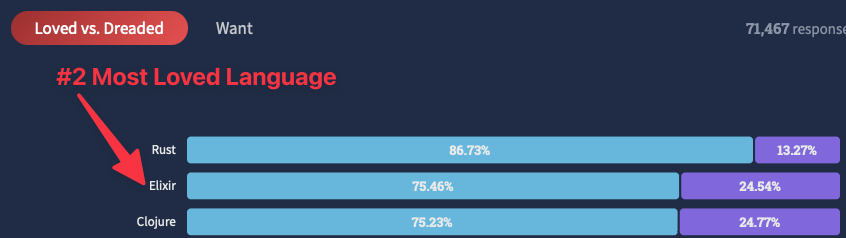
\includegraphics{./images/1.1-stackoverflowsurvey.png}

\begin{enumerate}
\def\labelenumi{\arabic{enumi}.}
\setcounter{enumi}{3}
\tightlist
\item
  A Clear Path to Production Building models on your machine is sweet,
  but what about when you're ready to go live? How much additional stuff
  is needed to turn your Python or R code into something that is
  production ready? How will you handle \ldots{}
\end{enumerate}

\begin{itemize}
\tightlist
\item
  Background Jobs
\item
  Crash Recovery
\item
  Long-Running Requests
\item
  Low Latency App State
\item
  Etc\ldots{}
\end{itemize}

What additional technologies will you have to include? Is the additional
complexity worth it?

In his book, Elixir In Action, Sasa Juric showed, in the table below,
that Elixir (built on top of Erlang) gives you all of these things for
free! 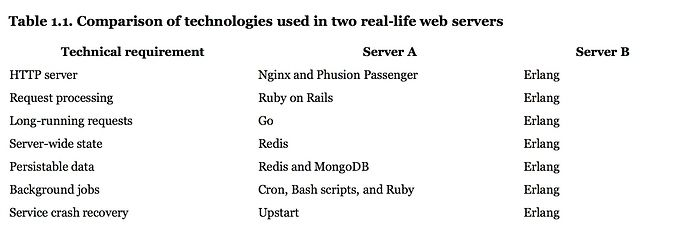
\includegraphics{./images/1.2-elixirinaction.jpeg}

Elixir already has a production-ready web framework named Phoenix. Do
you want to use your model in your website? Done. Do you want to deploy
your model results as an API for others to consume? No problem. And the
cool part is, Phoenix is \emph{The Most Loved Web Framework} according
to the Stack Overflow 2022 Survey (shown below).
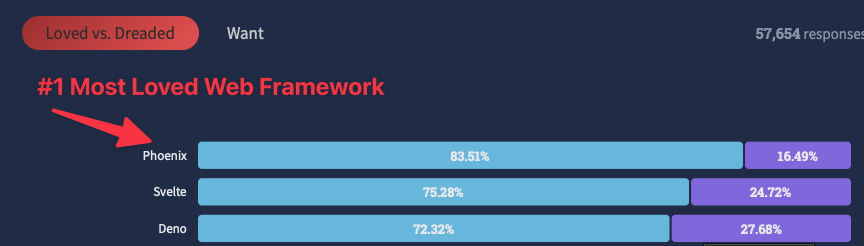
\includegraphics{./images/1.3-stackoverflowsurvey.png}

Elixir is turning itself into a one-stop-shop for all your Data Science
needs.

\hypertarget{setup-and-installation}{%
\section*{Setup and Installation}\label{setup-and-installation}}
\addcontentsline{toc}{section}{Setup and Installation}

If you're still with me, let's get the setup and install out of the way.
There are 3 ways to get up and going with Elixir and Livebook.

\begin{enumerate}
\def\labelenumi{\arabic{enumi}.}
\item
  If you have access to a computer, the easiest way to get up and going
  is selecting the Mac or Windows option and downloading the appropriate
  software for your computer. This requires zero setup. Once downloaded,
  simply install Livebook, and you're up and running. That's it!
  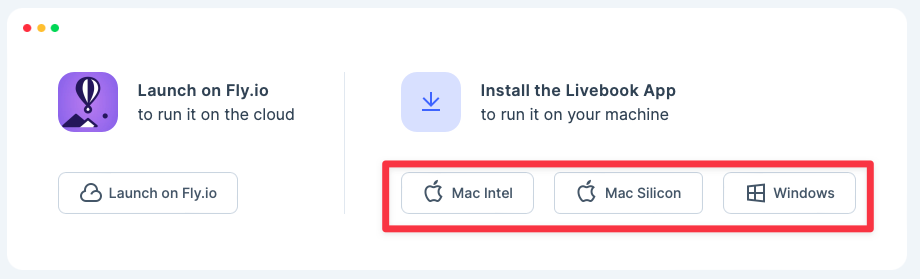
\includegraphics{./images/1.4-flyio.png}
\item
  If you want to work in the cloud, select the Fly.io option. This
  requires setting up an account and a few odds and ends. You should be
  up and running in under 5 minutes. No, I'm not lying. I actually did
  have a cloud version of Livebook going in under 5 minutes.
  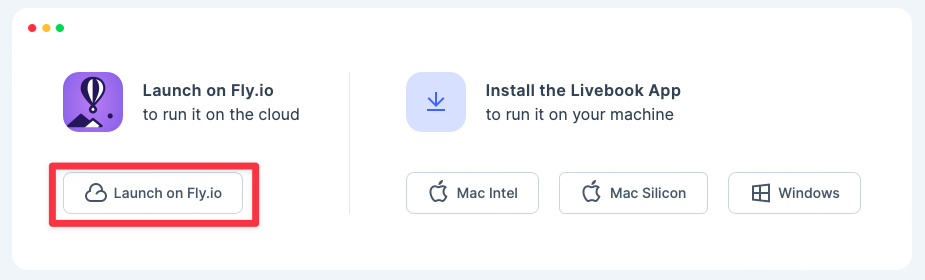
\includegraphics{./images/1.5-flyio.png}
\item
  If you'd like to manually install all the parts yourself, then you'll
  need to install Erlang, Elixir and run Escript to install Livebook.
  You can find the directions
  \href{https://github.com/livebook-dev/livebook\#installation}{here}.
\end{enumerate}

Finally, let's install the packages you'll need

\begin{Shaded}
\begin{Highlighting}[]
\ConstantTok{Mix}\OperatorTok{.}\NormalTok{install([}
\NormalTok{  \{}\VariableTok{:vega\_lite}\NormalTok{, }\StringTok{"\textasciitilde{}\textgreater{} 0.1.6"}\NormalTok{\},}
\NormalTok{  \{}\VariableTok{:kino}\NormalTok{, }\StringTok{"\textasciitilde{}\textgreater{} 0.6.2"}\NormalTok{\},}
\NormalTok{  \{}\VariableTok{:kino\_vega\_lite}\NormalTok{, }\StringTok{"\textasciitilde{}\textgreater{} 0.1.2"}\NormalTok{\},}
\NormalTok{  \{}\VariableTok{:explorer}\NormalTok{, }\StringTok{"\textasciitilde{}\textgreater{} 0.3.0"}\NormalTok{\}}
\NormalTok{])}
\end{Highlighting}
\end{Shaded}

\bookmarksetup{startatroot}

\hypertarget{summary}{%
\chapter{Summary}\label{summary}}

In summary, this book has no content whatsoever.

\bookmarksetup{startatroot}

\hypertarget{references}{%
\chapter*{References}\label{references}}
\addcontentsline{toc}{chapter}{References}

\hypertarget{refs}{}
\begin{CSLReferences}{0}{0}
\end{CSLReferences}

\bookmarksetup{startatroot}

\hypertarget{resources}{%
\chapter*{Resources}\label{resources}}
\addcontentsline{toc}{chapter}{Resources}

\begin{itemize}
\tightlist
\item
  \href{https://podcast.thinkingelixir.com}{Thinking Elixir Podcast}

  \begin{itemize}
  \tightlist
  \item
    \href{https://podcast.thinkingelixir.com/102}{Machine Learning}
  \item
    \href{https://podcast.thinkingelixir.com/104}{Exploring Data}
  \end{itemize}
\item
  \href{https://r4ds.had.co.nz/}{R for Data Science Book}
\end{itemize}



\end{document}
